Debido a la \textit{"intratabilidad"} del problema de la partición de grafos, como hemos comentado, no existe un algoritmo concreto que permita obtener en tiempo polinómico una solución óptima a la partición de cualquier grafo. Es por ello por lo que, los algoritmos codificados para este informe se basan en la metaheurística, con el objetivo de obtener soluciones de buena calidad en tiempos computacionales aceptables, a pesar de que los algoritmos metaheurísticos no garantizan que se vaya a obtener una solución óptima al problema.

En el siguiente apartado se describen los algoritmos Kernighan-Lin\cite{KernighanLin} (ver apartado \ref{Kernighan-Lin}), Specrtal Bisection (ver apartado \ref{Spectral-Bisection}) y Multilevel Spectral Bisection (ver apartado \ref{Multilevel-Spectral-Bisection}). Tres algoritmos que se diseñaron específicamente para la resolución del problema de la partición de grafos. Cualquiera de estos algoritmos proporciona una solución factible al problema, pudiendo ser esta óptima o no. El enfoque del informe radica en la partición de diferentes grafos en dos particiones usando estos tres algoritmos. 

Además de describir cada uno de los algoritmos, también se describirán algunos detalles sobre su codificación.
De ejemplo para describir cada codificación se ha utilizado un grafo inicial (ver Figura \ref{grafo}). Este grafo es un grafo no dirigido (ver Definición \ref{no_dirigido}) de diez nodos con pesos en sus aristas.

\begin{mydef}\label{no_dirigido}
	Un grafo no dirigido es un grafo (ver Definición \ref{def:grafo} ) donde: $V\neq \emptyset$ y $E\subseteq \{x\in \mathcal P(V):|x|=2\}$ es un conjunto de pares no ordenados de elementos de $V$. Un par no ordenado es un conjunto de la forma \{a , b\}, de manera que \{a, b\} = \{b, a\}. En los grafos, los conjuntos de pares no ordenados pertenecen al conjunto potencial de $V$, denotado $\mathcal P(V)$, y son de cardinalidad 2. 
\end{mydef}

\renewcommand{\figurename}{Figura}
\begin{figure}[h]
	\centering
	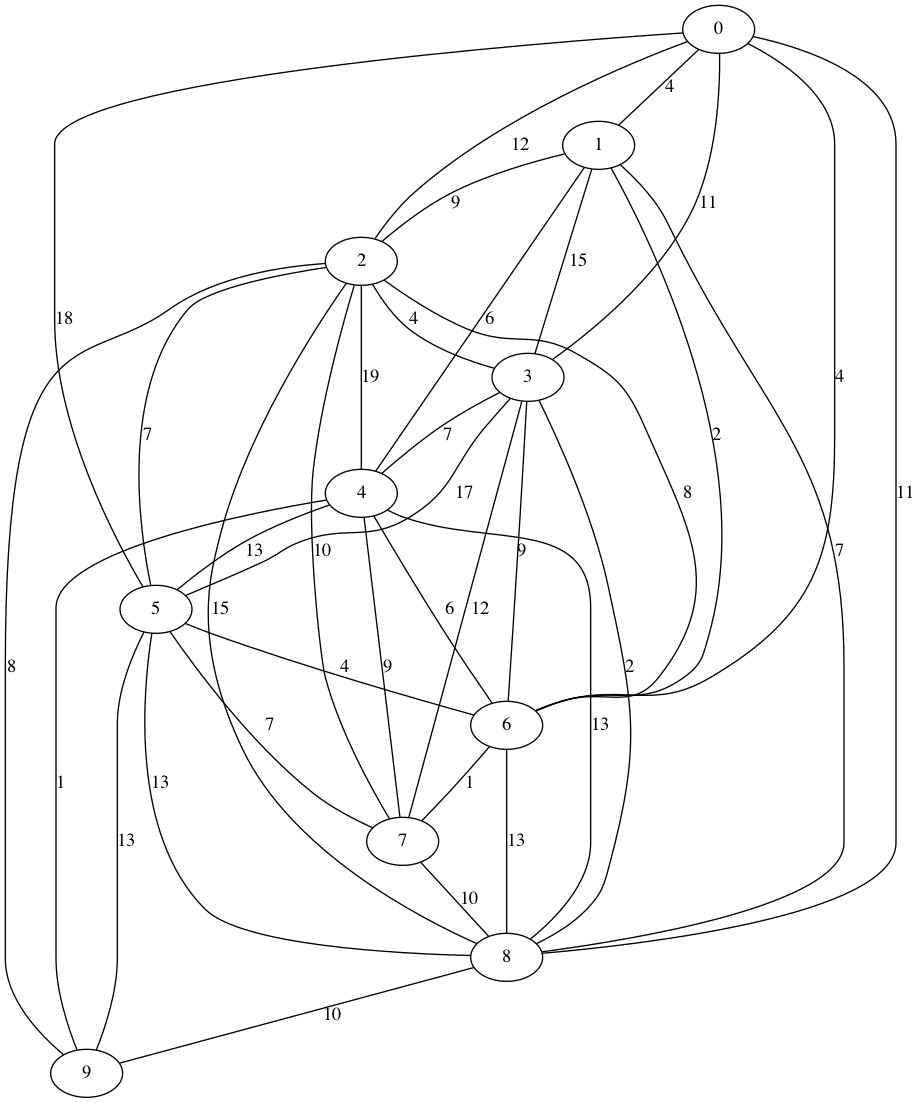
\includegraphics[scale=0.25]{Figures/10_dataset}
	\vspace{1mm}
	\caption{Grafo inicial.}
	\label{grafo}
\end{figure}

\newpage
\section{Kernighan-Lin}\label{Kernighan-Lin}

El algoritmo Kernighan-Lin\cite{KernighanLin}, a menudo abreviado como K-L, es uno de los primeros algoritmos de partición de grafos y fue desarrollado originalmente para optimizar la colocación de circuitos electrónicos en tarjetas de circuito impreso para minimizar el número de conexiones entre las tarjetas (circuitos VLSI\cite{KernighanLin}\cite{Ravikumar}).

El algoritmo es:

\begin{itemize}
	\setlength{\parskip}{0pt}
	\setlength{\itemsep}{0pt plus 1pt}
	\item \textbf{Iterativo}. Porque el grafo inicialmente ya está particionado, pero la aplicación del algoritmo intentará mejorar u optimizar la partición inicial. 
	\item \textbf{Voraz}. Porque el algoritmo hará cambios si hay un beneficio inmediato sin considerar otras formas posibles de obtener una solución óptima. Para ello, elige la opción óptima en cada paso con la esperanza de llegar a una solución general óptima.
	\item \textbf{Determinista}. Porque se obtendrá el mismo resultado cada vez que se aplique el algoritmo. 
\end{itemize}

El algoritmo K-L, como acabamos de describir, no crea particiones, sino que las mejora iterativamente. La idea original era tomar una partición aleatoria y aplicarle Kernighan-Lin\cite{KernighanLin}. Esto se repetiría varias veces y se elegiría el mejor resultado. Mientras que para grafos pequeños esto ofrece resultados razonables, es bastante ineficiente para tamaños de grafos más grandes.

Hoy en día, el algoritmo se usa para mejorar las particiones encontradas por otros algoritmos, tratando de mejorar las particiones mediante el intercambio de nodos vecinos. Por tanto, complementa muy bien otro tipo de algoritmos como por ejemplo los que realizan una partición espectral (ver sección \ref{Spectral-Bisection}).

\subsection{Descripción}

El objetivo del algoritmo es dividir el conjunto de vértices $V$ de un grafo no dirigido (ver Definición \ref{no_dirigido}) en dos subconjuntos disjuntos (ver Definición \ref{disjuntos}) $A$ y $B$ de igual tamaño, de una manera que minimice la suma $T$ de los pesos del subconjunto de aristas que cruzan de $A$ a $B$. El algoritmo mantiene y mejora una partición, en cada iteración usando un algoritmo voraz (ver Definición \ref{voraz}), empareja los vértices de $A$ con los vértices de $B$, de modo que al mover los vértices emparejados de una partición a la otra se maximiza la ganancia, que mide cuánta "información" nos brinda la función objetivo. Después de emparejar los vértices y maximizar la ganancia, crea un subconjunto de los pares de los vértices elegidos para tener el mejor efecto sobre la calidad de la solución $T$. Dado un grafo con n vértices, cada iteración del algoritmo se ejecuta en el tiempo $O({n}^2 \, log \, n)$.

\begin{mydef}\label{disjuntos}
	$A$ y $B$ son dos subconjuntos disjuntos si $A \cup B$ y $A \cap B \neq 0$.
\end{mydef}

\begin{mydef}\label{voraz}
	Dado un conjunto finito $C$, un algoritmo voraz devuelve un conjunto $S$ tal que $S\subseteq C$ y que además cumple con las restricciones del problema inicial. A cada conjunto $S$ que satisfaga las restricciones y que logra que la función objetivo se minimice o maximice (según corresponda) diremos que $S$ es una solución óptima. 
\end{mydef}

Más detalladamente, sea $a$ un elemento del subconjunto $A$ y $b$ un elemento del subconjunto $B$, para cada $a \in A$, $I_{a}$ es el coste interno de a, es decir, la suma de los pesos de las aristas entre a y otros nodos en $A$. Y $E_{a}$ es el coste externo de a, es decir, la suma de los pesos de las aristas entre a y los nodos en $B$. De manera similar, se define $I_{b}$ y $E_{b}$ para cada $b \in B$.

Así podemos decir que existe una diferencia $D$ entre la suma de los costes externos e internos $s$. Si formalizamos obtenemos:

\begin{center}
	$D_{s} = E_{s} - I_{s}$
\end{center}

Y entonces si $a$ y $b$ se intercambian, la ganancia se calcula como:

\begin{center}\label{ganancia}
	$T_{antigua} - T_{nueva} = D_{a} + D_{b} - 2c_{a, b}$ 
\end{center}

donde $c_{a, b}$ es el coste de las aristas posibles entre $a$ y $b$.

El algoritmo intenta encontrar una solución óptima de operaciones de intercambio entre los elementos de $A$ y $B$ que maximice la ganancia ($T_{antigua} - T_{nueva}$) y luego ejecuta las operaciones, produciendo una partición del grafo en $A$ y $B$.

Con estos dos conceptos, podemos describir la primera iteración del algoritmo usando el pseudocódigo en \cite{Ravikumar}.

\begin{lstlisting}[frame=single] 
function Kernighan-Lin(G(V, E)) is
 determine a balanced initial partition of the nodes into sets A and B

 do
  compute D values for all a in A and b in B
  let gv, av, and bv be empty lists
  for n := 1 to |V| / 2 do
    find a from A and b from B, such that gain is maximal
    remove a and b from further consideration in this pass
	add g to gv, a to av, and b to bv
	update D values for the elements of A = A \ a and B = B \ b
  end for
  find k which maximizes g_max, the sum of gv[1], ..., gv[k]
  if g_max > 0 then
    Exchange av[1], av[2], ..., av[k] with bv[1], bv[2], ..., bv[k]
  until (g_max <= 0)  
    
return G(V, E) 
\end{lstlisting}

Entonces, en cada iteración, el algoritmo K-L intercambia pares de vértices para maximizar la ganancia. Y continúa haciéndolo hasta que se intercambian todos los vértices de la partición más pequeña. 

Una gran ventaja del algoritmo es que no se detiene incluso aceptando ganancias negativas, sigue esperando que las ganancias posteriores sean más grandes y que el tamaño de la suma de los pesos de las aristas se reduzca hasta que se intercambian todos los vértices de la partición más pequeña. Esta capacidad es una característica crucial. Aunque esta capacidad sea crucial, el algoritmo tiene unas cuantas desventajas:

\begin{itemize}
	\item Los resultados son aleatorios porque el algoritmo comienza con una partición aleatoria.
	\item Computacionalmente es un algoritmo lento.
	\item Solo se crean dos particiones del mismo tamaño.
	\item Las particiones deben tener el mismo tamaño para que el algoritmo no intente encontrar soluciones óptimas que ya existan.
	\item No resuelve muy bien los problemas con las aristas ponderadas.
	\item La solución dependerá en gran medida de la primera partición.
\end{itemize}

C. Fiduccia y R. Mattheyses realizaron importantes avances prácticos en \cite{FiducciaMattheyses}, quienes mejoraron el algoritmo de  Kernighan-Lin\cite{KernighanLin} de tal manera que, cada partición se ejecuta en $O({n}^2)$, en lugar de $O({n}^2 \, log \, n)$. La reducción se logra en parte eligiendo nodos individuales para intercambiar en lugar de parejas de vértices.

\subsection{Ejemplo de codificación}

Existen muchas variaciones del algoritmo K-L que a menudo intercambian el tiempo de ejecución con la calidad, o generalizan el algoritmo a más de dos particiones. En este caso, para la codificación del algoritmo se ha utilizado la libraría de Python: \href{https://networkx.github.io/documentation/stable/reference/algorithms/generated/networkx.algorithms.community.kernighan_lin.kernighan_lin_bisection.html}{NetworkX}. El algoritmo divide un grafo en dos particiones usando el algoritmo Kernighan-Lin\cite{KernighanLin}. Es decir, divide un grafo en dos conjuntos intercambiando iterativamente pares de nodos para reducir el peso de las aristas entre los dos conjuntos.

\begin{mydef}\label{NetworkX}
	NetworkX es un paquete de Python para la creación, manipulación y estudio de la estructura, dinámica y funciones de los grafos. 
\end{mydef}

Por ejemplo, en una ejecución de la codificación, donde la entrada es el grafo de la Figura \ref{grafo}, y después de una partición inicial, podemos obtener los subconjuntos: A = \{3, 4, 6, 8, 9\} y B = \{0, 1, 2 , 5, 7\}. Estos subconjuntos son del mismo tamaño y sus elementos están ordenados.

En esta ejecución, los pasos que sigue el algoritmo son los siguientes:

\begin{itemize}
	\item Dibuja una línea que separa el grafo en dos particiones con el mismo número de vértices en cada partición.
	\item Cuenta la cantidad de aristas que cruzan la línea. Este número se llama \textit{"cut-size"} y el objetivo es disminuirlo, es decir, disminuir el número de conexiones entre los vértices del grafo.
	\item Encuentra el coste de todos los vértices en el grafo, buscando el número de conexiones que cada vértice tiene dentro de su propia partición y restando eso del número de conexiones que cada vértice tiene con vértices en la otra partición.
	\item Determina la ganancia máxima intercambiando dos nodos. La ecuación de ganancia es la que se muestra en \ref{ganancia}.
	\item Intercambia los dos nodos con la ganancia máxima. Si se han calculado todas las ganancias de emparejamiento de todos los nodos y la ganancia máxima es igual a cero o negativa, los nodos con la ganancia más alta aún deberán intercambiarse.
	\item Resta la ganancia del \textit{"cut-size"} original para obtener el nuevo \textit{"cut-size"}.
	\item Cambia los nodos que se han intercambiado.
	\item Repite estos pasos hasta que la ganancia máxima es cero o negativa.
\end{itemize}

\newpage
\section{Spectral Bisection}\label{Spectral-Bisection}

\subsection{Descripción}

\subsection{Ejemplo de codificación}

Después de la partición obtenemos los conjuntos: A = \{1, 2, 3, 4, 6, 9\} y B = \{0, 8, 5, 7\}.

Los conjuntos no son del mismo tamaño. No están ordenados.

\newpage
\section{Multilevel Spectral Bisection}\label{Multilevel-Spectral-Bisection}

El particionamiento de grafos por multilevel es un método moderno que reduce el tamaño de las particiones del grafo con la combinación de los vértices y las aristas sobre varios niveles, creando particiones del grafo cada vez más pequeñas y extensas con muchas variaciones y combinaciones de diferentes métodos.

\subsection{Descripción}\label{msb_description}

Y esta es, en líneas generales, la descripción de uno de los algoritmos más exitosos para el problema de partición de grafos.

\subsection{Ejemplo de codificación}

El algoritmo Multilevel Spectral Bisection (MSB) descrito en la sección \ref{msb_description} ha resultado ser muy eficiente (ver sección \ref{chapter:Comparativa}). En MSB, se transfiere información aproximada sobre el segundo \textit{eigenvector} del grafo original entre niveles, mejorando esta información en cada nivel y finalmente, se usa otra vez el \textit{eigenvector} para dividir el grafo. 

Se muestra el pseudocódigo del algoritmo a continuación:

\begin{lstlisting}[frame=single] 
Function ML-Partition(G)

  If G is small enough then
    Find partition (V1, V2) of G in some way
    
  else

    Construct a smaller approximation G'
    (V1', V2') = ML-Partition(G')
    (V1", V2") = Project-partition-up (V1', V2')
    (V1, V2)   = Refine-partition (V1", V2")

endif

Return (V1, V2)
\end{lstlisting}

La misma idea se puede usar para dividir el grafo en \textit{p} partes a la vez. En realidad, hay toda una familia de algoritmos que puede dividir grafos en \textit{p} partes a la vez. Algunos de estos algoritmos se encuentran implementados en paquetes de software como Chaco\cite{Chaco}, METIS\cite{MeTis} o WGPP\cite{WGPP}.

Para la codificación del algoritmo se escogió la librería escrita en C de \href{http://glaros.dtc.umn.edu/gkhome/metis/metis/overview}{METIS} junto con NetworkX (ver Definición\ref{NetworkX}). Concretamente, la librería que se ha utilizado de Python es: \href{https://networkx-metis.readthedocs.io/en/latest/reference/generated/nxmetis.partition.html#nxmetis.partition}{NetworkX-METIS}. \textit{NetworkX-METIS} es un complemento para el paquete Python de \textit{NetworkX} que usa METIS\cite{MeTis} para la partición de grafos. Los algoritmos implementados en METIS se basan en los esquemas de bisección multinivel.

Las características clave de METIS son las siguientes:

\begin{itemize}
	\item Proporciona particiones de alta calidad. Los experimentos con una gran cantidad de nodos muestran que METIS produce particiones que son consistentemente mejores que las producidas por otros algoritmos ampliamente utilizados. Las particiones producidas por METIS son consistentemente 10\% a 50\% mejores que las producidas por algoritmos de partición espectral.
	\item Es extremadamente rápido. Los experimentos en una amplia gama de grafos han demostrado que METIS es de uno a dos órdenes de magnitud más rápido que otros algoritmos de partición ampliamente utilizados.
\end{itemize}

METIS es un algoritmo de partición de grafos que se enfoca en minimizar el número de aristas cruzadas de cada partición y distribuir la carga de trabajo de manera uniforme entre las particiones. Con METIS, los gráficos se dividen en tres fases. La primera fase es la fase de engrosamiento, la segunda la fase de partición y la tercera y última fase la fase de no engrosamiento (Figura X). La fase de particionamiento contiene particiones bi-particionadas y K-way. A diferencia de la partición K-way, la bi-partición se realiza de forma recursiva. Las subseccion a continuación contienen una explicación más extensa de estas diversas fases.

Por ejemplo, en una ejecución de la codificación, la entrada es el grafo de la Figura \ref{grafo}. El resultado de aplicar el algoritmo codificado son los conjuntos: A = \{0, 1, 3, 7, 8\} y B = \{2, 4, 5, 6, 9\}. Estos conjuntos tienen el mismo tamaño y sus elementos están ordenados.